\section{Major Components in our project}

\subsection{Simple Pendulum}
\begin{wrapfigure}{r}{0.4\textwidth}
	\caption{A picture of simple pendulum}
	\begin{center}
	 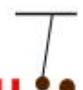
\includegraphics[width=0.2\textwidth]{pendulum.jpg}%
	 \end{center}
	
\end{wrapfigure}

\begin{frame}
\centering

The formula for time period of pendulum is:
\begin{equation}
\\
\\
	T = 2\pi \sqrt {\frac{l}{g}}
	\\
	\\
\end{equation}
\begin{flushleft}
 -$ l $ is the length of the string from the center of the bob to the pivot\\ 
- $ g $ is the acceleration due to gravity\\
\end{flushleft}
Our project starts with an oscillating simple\\ pendulum giving impulse to a domino placed\\ on one side of it and a ball placed on other side of it.
\end{frame}
\\
\\
\\
\\
\\
%%%%%%%%%%%%%%%%%%%%%%%%%%%%%%%%%%%%%%%%%%%%%%%%%%%%%%%%%%%%%%%
\subsection{Conveyor belt}
\begin{wrapfigure}{r}{0.4\textwidth}
	\caption{A picture of conveyor belt}
	\centering
	 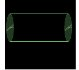
\includegraphics[width=0.2\textwidth]{conveyorbelt.jpg}%
\end{wrapfigure}
\begin{frame}
\centering
\\
Conveyor in our project is used to carry\\ a block which triggers a mechanism . \\
Here whenever an object falls on\\ the conveyor belt we used sensors to \\detect the object and give it a force to the \\left or right accordingly.\\We introduced there two rotating motors to\\ give the effect of conveyor belt. 
\end{frame}

\newpage
%%%%%%%%%%%%%%%%%%%%%%%%%%%%%%%%%%%%%%%%%%%%%%%%%%%%%%%%%%%%%%%
\subsection{Pressure transfering system}
\begin{wrapfigure}{r}{0.4\textwidth}
	\caption{A picture of pressure tranfering system}
	\centering
	 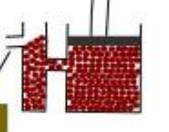
\includegraphics[width=0.2\textwidth]{pasc.jpg}%
\end{wrapfigure}
\begin{frame}
\centering
\\
\\
In this system when we give pressure on \\the large surface the prssure gets\\ equally distributed and the popcorn\\ on the otherside start falling into \\the container.
\end{frame}
\\
\\
\\
\\
%%%%%%%%%%%%%%%%%%%%%%%%%%%%%%%%%%%%%%%%%%%%%%%%%%%%%%%%%%%%%%%
\subsection{Balloon System}
\begin{wrapfigure}{r}{0.4\textwidth}
	\caption{A picture of balloon system}
	\centering
	 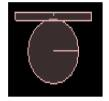
\includegraphics[width=0.2\textwidth]{balloon.jpg}%
\end{wrapfigure}
\begin{frame}
\centering
\\
\\
We made this balloon system simulation\\by introducing the negative gravity because of \\which they move upward to trigger \\the container.
\end{frame}
\\
\\
%%%%%%%%%%%%%%%%%%%%%%%%%%%%%%%%%%%%%%%%%%%%%%%%%%%%%%%%%%%%%%
\subsection{Rotating Motor}
\begin{wrapfigure}{r}{0.4\textwidth}
	\caption{A picture of rotating motor}
	\centering
	 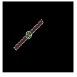
\includegraphics[width=0.2\textwidth]{motor.jpg}%
\end{wrapfigure}
\begin{frame}
\centering
\\
\\
We have introduced RevoluteJointDef and enabled \\the motor property.We have given that\\ motor an angular speed and required torque\\ accordingly.
\end{frame}
\\
\\
%%%%%%%%%%%%%%%%%%%%%%%%%%%%%%%%%%%%%%%%%%%%%%%%%%%%%%%%%%
\subsection{Hinge system}
\begin{wrapfigure}{r}{0.4\textwidth}
	\caption{A picture of hinge system}
	\centering
	 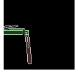
\includegraphics[width=0.2\textwidth]{hingesystem.jpg}%
\end{wrapfigure}
\begin{frame}
\centering
\\
\\
We used Revolute Joint to give the effect of\\ hinge.It takes one anchor and two objects\\ and connects the two objects with the\\ thread through the point.We defined\\ one of the objects as a dynamic rod and other\\ as a small static object with the anchor point\\ on itself which gives the effect\\ of hinge.
\end{frame}
\\
\\
\newpage
%%%%%%%%%%%%%%%%%%%%%%%%%%%%%%%%%%%%%%%%%%%%%%%%%%%%%%%%%%%%%
\subsection{Pulley system}
\begin{wrapfigure}{r}{0.4\textwidth}
	\caption{A picture of pulley system}
	\centering
	 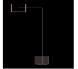
\includegraphics[width=0.2\textwidth]{pulleysystem.jpg}%
\end{wrapfigure}
\begin{frame}
\centering
\\
\\
Pulley joints are used to make this hinge system\\which takes two anchors and two objects and \\connects the two objects with the thread\\ through two points giving the effect\\ of a common balance.
\end{frame}
\\
\\
%%%%%%%%%%%%%%%%%%%%%%%%%%%%%%%%%%%%%%%%%%%%%%%%%%%%%%%%%%%%%






